\begin{animateinline}[final,loop,controls,poster=last]{1}
    \multiframe{8}{iCOUNT=00+01}{
       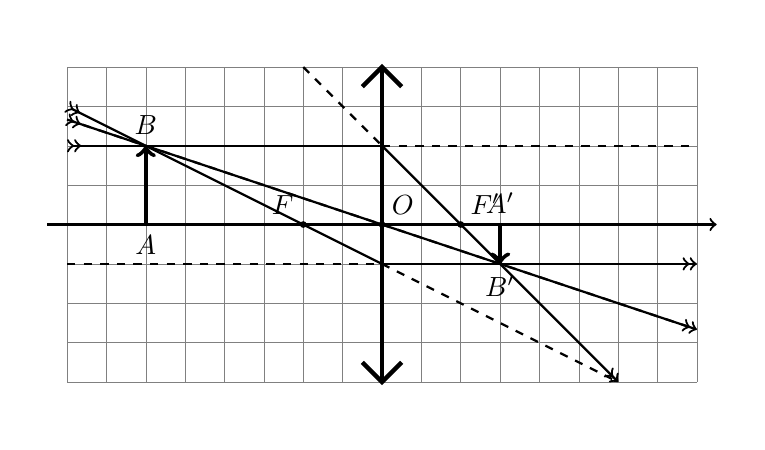
\begin{tikzpicture}[scale=0.5]
    \clip (-9,-5) rectangle (9,5) ;
    \draw [help lines] (-8,-4) grid [step=1] (8,4) ; %% Le quadrillage
    \draw [->,thick] (-8.5,0) -- (8.5,0) ; %% L'axe optique
    \draw [ultra thick] (0,-4) -- (0,4)  ; %% Le corps du syst�me 

    \draw [ultra thick] (-0.5,-3.5) -- (0,-4) -- (0.5,-3.5)
                         (-0.5,3.5) -- (0, 4) -- (0.5,3.5) ;
    \filldraw [black] (2.0,0) circle (2pt) node [above right] {$F'$};
    \filldraw [black] (-2.0,0) circle (2pt) node [above left] {$F$} ;
    \filldraw [black] (0,0) circle (2pt) node [above right] {$O$} ;
    
      \draw [->,ultra thick] (-6.0,0) node [below] {$A$} -- (-6.0,2.0) node [above] {$B$} ;
    
    \ifthenelse{\iCOUNT > 6}{
      \draw [->,ultra thick] (3.0,0) node [above] {$A'$} -- (3.0,-1.0) node [below] {$B'$} ;
      }{}
    
    \ifthenelse{\iCOUNT > 0}{  
    \draw [thick ,>>-] (-8,2.0) -- (0,2.0);
    \draw [thick , dashed] (0,2.0) -- (8,2.0);
    }{}
    
    \ifthenelse{\iCOUNT > 1}{
    \draw [thick , dashed] (-2.0,4.0) -- (0,2.0);
    \draw [thick ,->>] (0,2.0) -- (6.0,-4.0);
    }{}
    
    \ifthenelse{\iCOUNT > 2}{
    \draw [thick ,>>-] (-8,2.667) -- (0,0.0);
    \draw [thick , dashed] (0,0.0) -- (8,-2.667);
    }{}
    
    \ifthenelse{\iCOUNT > 3}{
    \draw [thick , dashed] (-8,2.667) -- (0,0.0);
    \draw [thick ,->>] (0,0.0) -- (8,-2.667);
    }{}
    
    \ifthenelse{\iCOUNT > 4}{
    \draw [thick ,>>-] (-8,3.0) -- (0,-1.0);
    \draw [thick , dashed] (0,-1.0) -- (6.0,-4.0);
    }{}
    
    \ifthenelse{\iCOUNT > 5}{
    \draw [thick , dashed] (-8,-1.0) -- (0,-1.0);
    \draw [thick ,->>] (0,-1.0) -- (8,-1.0);
    }{}
    
       \end{tikzpicture}
    }
\end{animateinline}

